\subsection{SCIPP Tracking R\&D}
SCIPP has been involved in Linear Collider tracking R\&D for a number of years, and its work has led to the development of a refined understanding of several generic tracking issues with potential applications for Linear Collider detectors. These include the use of resistive strips and dual-end readout for the determination of the longitudinal coordinate of the charge deposition on narrow electrodes [1] and limitations on silicon microstrip ladder length for precision narrow-strip sensors [2]. These studies are in fact dependent only on the properties of the electrode that collects the signal and propagates it to the readout electronics, and thus are independent of the sensor technology that generates the signals. Thus, this work may have relevance to detection issues across a wide array of fields.
Ongoing tracking R\&D is focused on the further development of the Long Shaping-Time Front End (LSTFE) microstrip readout ASIC. This properties of this ASIC have been explicitly optimized for the readout of long ladders of silicon strip sensors that are motivated by the need for precise low-mass central tracking for a Linear Collider Detector. With a small and straightforward change to the shaping properties of the ASIC, it could be reoptimized for use for the short strips and high occupancy that would be expected for ILC forward-tracking applications.
Similar to most ILC-oriented readout designs, the LSTFE features a long shaping time optimized to reduce voltage-referenced readout noise, as appropriate for narrow-strip, long-ladder applications. Unique to the LSTFE design, however, is the use of time-over-threshold readout to estimate the analog pulse-height generated by through-going subatomic particles. A pule-development and readout simulation developed at SCIPP suggested that the intrinsic statistical fluctuations of the charge-deposition process in 300 µm of silicon obviate the need for a precise measurement of deposited charge. A simulation of the centroid-finding (position-resolution) uncertainty provided by time-over-threshold readout showed little degradation relative to that provided by an exact measurement of deposited charge.
On the other hand, there are several advantages offered by the use of time-over-threshold readout. It is very simple to implement within a digital back-end to the LSTFE’s analog front end (the implementation would be on the same chip as the front-end readout), requiring only a measurement of the number of clock counts that the given channel is over threshold, and then the assembly and transmission of a single data word containing the time of the upward transition, the time over threshold after the transition, and the channel number. This happens in real time and is driven immediately off the chip into the DAQ, eliminating the need for buffering and ADC conversion. In particular, there is no limit to the rate at which particles can be detected other than the return-to-baseline of the analog signal, and so the data-accumulation rate capability of the device is very high. In addition, for forward tracking, for which short strips are envisioned, the shaping time can be shortened significantly. This will further improve the rate capability of the LSTFE readout, making it an excellent choice for the high-occupancy forward region.
Figure 1 shows the measured fractional charge uncertainty for the LSTFE prototype ASIC; for depositions expected from minimum-ionizing particles (1-4 fC) the fractional charge measurement uncertainty is approximately 15\%, which is small compared to the intrinsic fluctuations that arise from the deposition process.
\begin{figure}
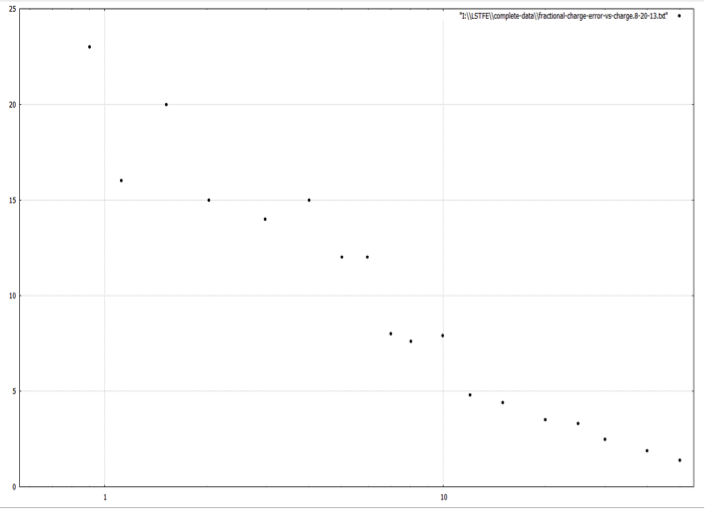
\includegraphics{SCIPPTracking}
\caption{Fractional pulse-height uncertainty (percent) versus injected charge (fC) for the LSTFE front-end ASIC.
The development of this ASIC has been done solely at the Santa Cruz Institute for Particle Physics (SCIPP) within the University of California at Santa Cruz, and while slowed significantly due to the loss of support for Linear Collider Detector R\&D, continues within SCIPP. Tasks that remain in developing a chip suitable for use in a Linear Collider Detector include the development of the digital back end; significant progress has already been made in defining the architecture of this section of the chip and in implementing this architecture in prototype form on an FPGA. Power cycling (switching the chip into a low-power quiescent mode for most of the 199 ms between beam crossings) also needs to be implemented.}
\end{figure}
 

References
[1] J. K. Carman et al., Longitudinal Resistive Charge Division in Multi-Channel Silicon Strip Sensors, Nulcear Inst. and Methods in Physics Research A579 (2007), pp 595-598.
[2] K. Collier et al., Microstrip Electrode Readout Noise for Load-Dominated Long Shaping-Time Systems, Nuclear Inst. and Methods in Physics Research, A729 (2013), pp. 127-132.
